\chapter{The strong coupling constant $\alpha_s$}

Spectroscopy studies, in addition to testing QCD, allow the determination of some of the fundamental parameters of the SM, i.e., the coupling $\alpha_s$ and the quark masses. To determine $\alpha_s$, one needs to know not only its strength but also the energy scale $Q$ at which the coupling is measured. The calculation of $\alpha_s$, in general, proceeds as follows. One chooses a quantity $O$ that can be measured very accurately, either in high energy experiments or via non-perturbative methods on the lattice, and for which a perturbative expansion is known, i.e.,
\begin{equation}
O = \sum_n A_n \alpha_s^n(Q),
\end{equation}
where the $A_n$ are the perturbative coefficients. Inverting this relation gives $\alpha_s(Q)$.

One promising lattice approach for calculating $\alpha_s$ has been pioneered by the NRQCD collaboration [110]. They examine several short-distance $O$, like the expectation value of small Wilson loops, that can be calculated very accurately on the lattice and for which perturbative expansions are known to at least $O(\alpha_s^2)$. The scale $Q$ characterizing these lattice observable is typically of the form $Q = C/a$ where $a$ is the lattice spacing and $C$ is a constant that needs to be fixed. They determine $C$ relevant to $O$ by evaluating the mean momentum flow in the perturbative expressions for these quantities. The scale $1/a$ is fixed using level splittings in quarkonia. In particular they use the spin-averaged S-P and the 1S-2S splittings in the Upsilon system. The advantage of using these splittings is that they show negligible sensitivity to the precise tuning of the bottom quark mass, and the corrections due to light quark loops are expected to be small.

Finally, to convert from $\alpha_s$ in the lattice scheme to $\alpha_{\overline{\mathrm{MS}}}$ they use the two loop relation, and include reasonable estimates of the $\alpha_s^3$ term in the error analysis. Their final estimate
\begin{equation}
\alpha_{\overline{\mathrm{MS}}}(M_Z) = 0.1174(24)
\end{equation}
includes quenching uncertainties. This remarkably precise result is consistent with the world average of experimental determinations, $\alpha_s = 0.118(3)$, as shown in Fig.~\ref{fig:33}.

An alternate method for measuring $\alpha_s$ has been carried out by the ALPHA collaboration [182]. In their method, called the Schr\"odinger functional approach, $\alpha_s$ is defined by measuring the response of the lattice system to an external field. They fix the lattice scale $a$ using the force at some fixed distance ($R_0 = 0.5$ fermi). They evolve their coupling to a very high scale using a non-perturbative renormalization group stepping procedure. At this high scale they define $\Lambda^{(0)}_{\overline{\mathrm{MS}}}$ using the two loop relation and include the three loop uncertainty, which is small, in error estimates. They have completed the calculation for the quenched theory with the result $\Lambda^{(0)}_{\overline{\mathrm{MS}}} = 251(21)$~MeV, and are now doing the $n_f = 2$ simulations [182]. The corresponding value $\alpha_{\overline{\mathrm{MS}}}(90~\mathrm{GeV}) = 0.0818(10)$ is lower than in nature. This difference is attributed to having neglected sea quark effects.

\begin{figure}[htbp]
\centering
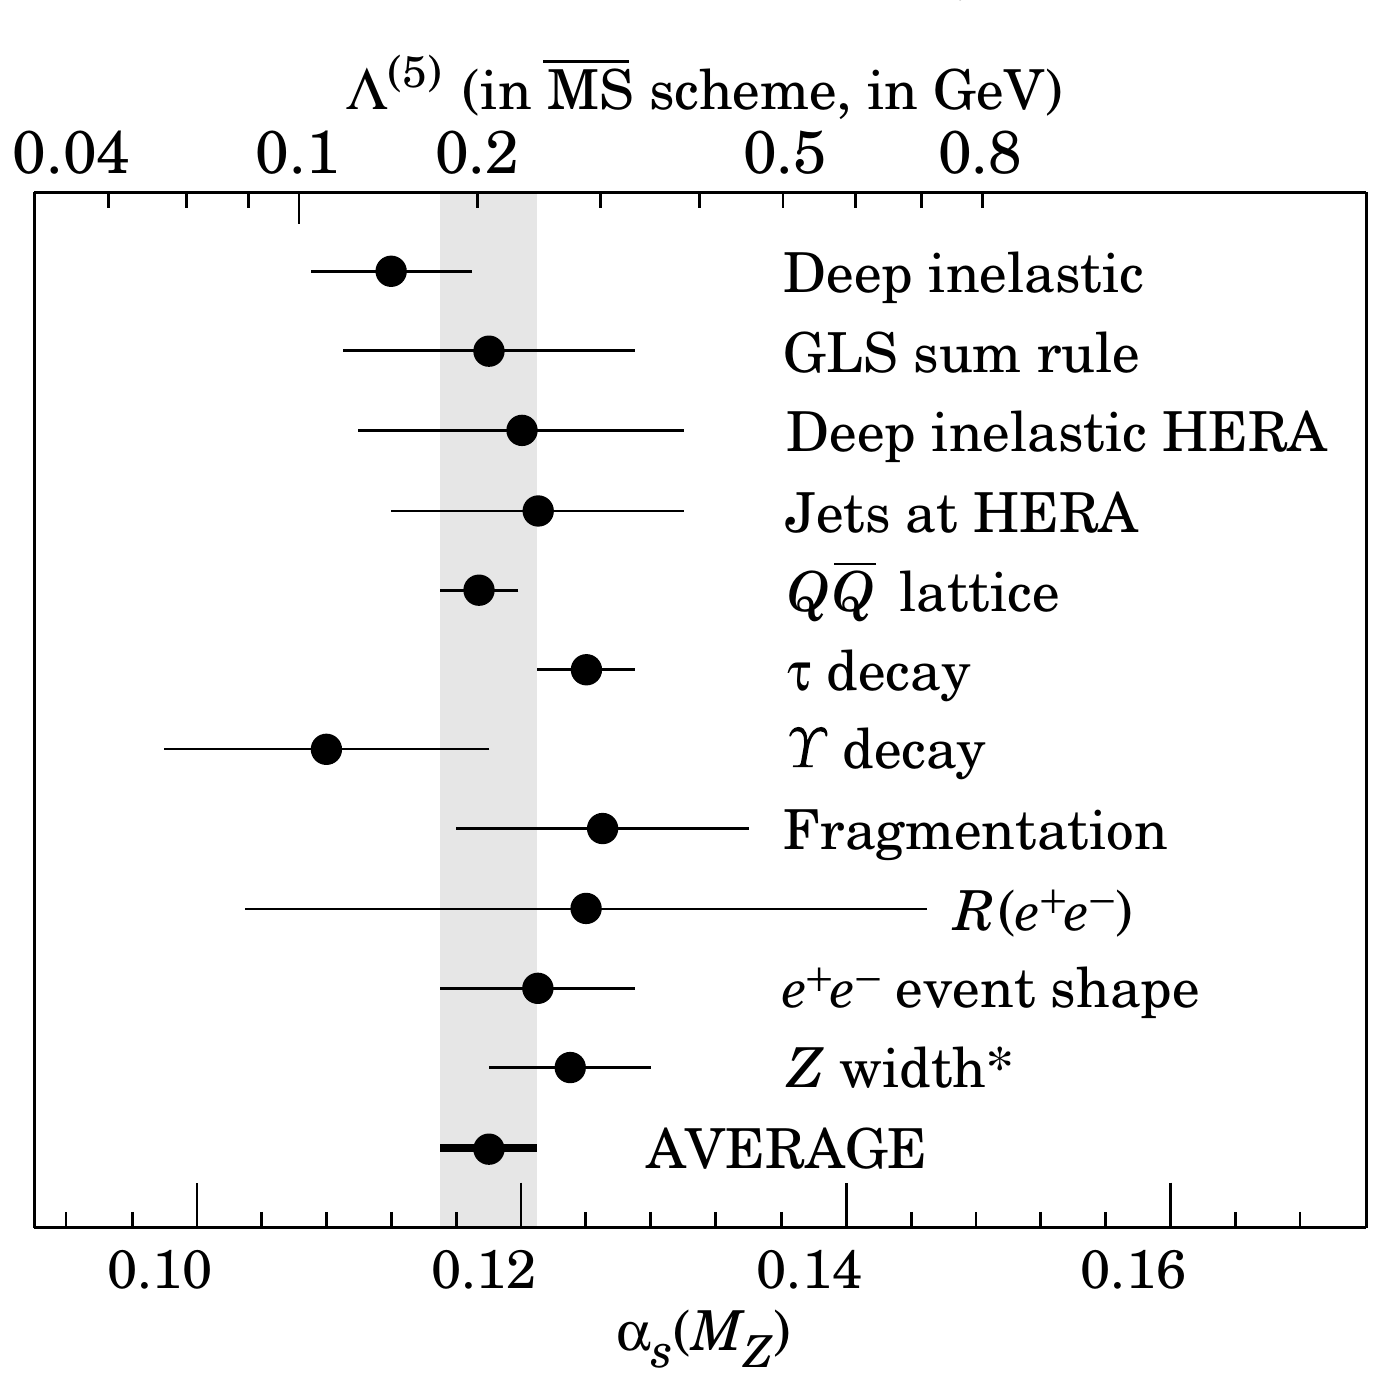
\includegraphics[width=0.8\textwidth]{images/fig33.png}
\caption{Summary of the values of $\alpha_s(M_Z)$ and $\Lambda^{(5)}$ (the QCD scale for 5 active quark flavors) extracted from various processes. These are ordered from top to bottom by increasing energy scale of measurements. This figure is reproduced from the 1996 Review of Particle Physics, updated to show the latest lattice result, $\alpha_{\overline{\mathrm{MS}}}(M_Z) = 0.1174 \pm 0.0024$. It is a remarkable confirmation of QCD that the $\alpha_s$ extracted from processes at different scales has the same value.}
\label{fig:33}
\end{figure}

A similar low value is obtained in the NRQCD analyses if no corrections are made for the quenched approximation. For details of the Schr\"odinger functional method see the lectures by Prof.~L\"uscher at this school.
